\documentclass[tikz,border=10pt]{standalone}

\usepackage{tikz}
\usetikzlibrary{positioning}
\usetikzlibrary{shapes,arrows,backgrounds,fit,shapes.geometric,calc}
\usetikzlibrary{pgfplots.groupplots}
\usepackage{pgfplots}
\usepackage{pgfplotstable}
\usepackage{listings}
\usepackage{lstautogobble}
\usepackage{color}

\tikzset{
    %Define standard arrow tip
    >=stealth',
    % Define arrow style
    pil/.style={
           ->,
           thick,
           shorten <=2pt,
           shorten >=2pt,}
}
\begin{document}
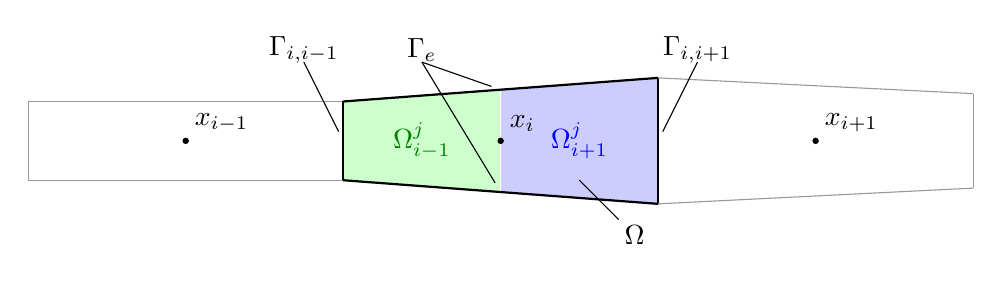
\begin{tikzpicture}[outer sep = 0pt]

%%%%%%%%%%%%%%%%%%%%%%%%%%%%%%%%%

% axis
%\draw [pil, very thin] (-3.4,0) -- ( 3.5, 0);
%\draw [pil, very thin] (-3.2,-0.2) -- (-3.2, 0.5);

% left sub CV
\filldraw[white,fill=green!20] (-2,-0.5) -- (-2,0.5) -- (0,0.65) -- (0,-0.65) -- cycle;
\filldraw[white,fill=blue!20] (0,-0.65) -- (0,0.65) -- ( 2, 0.8) -- ( 2, -0.8) -- cycle;

% left volume
\draw [white!60!black] (-6,-0.5) -- (-6, 0.5);
\draw [white!60!black] (-6,-0.5) -- (-2,-0.5);
\draw [white!60!black] (-6, 0.5) -- (-2, 0.5);

% central volume
\draw [thick] (-2,-0.5) -- (-2, 0.5);
\draw [thick] (-2, 0.5) -- ( 2, 0.8);
\draw [thick] (-2,-0.5) -- ( 2,-0.8);
\draw [thick] ( 2,-0.8) -- ( 2, 0.8);

% right volume
\draw [white!60!black] ( 2,-0.8) -- ( 6,-0.6);
\draw [white!60!black] ( 2, 0.8) -- ( 6, 0.6);
\draw [white!60!black] ( 6,-0.6) -- ( 6, 0.6);

%\coordinate [label=above right:{\tiny$x_i$}] (B) at (0,0);
\node [] (L) at (-4, 0) {};
\node [] (C) at ( 0, 0) {};
\node [] (R) at ( 4, 0) {};

% nodes that define the centre of each face
\node [] (Lface) at (-2, 0) {};
\node [] (Rface) at ( 2, 0) {};
\node [] (Tface) at ( 0, 0.65) {};
\node [] (Bface) at ( 0,-0.65) {};

% centroids
\path (L) node [shape=circle, draw, fill=black, scale=0.2] {}
      (C) node [shape=circle, draw, fill=black, scale=0.2] {}
      (R) node [shape=circle, draw, fill=black, scale=0.2] {};

\path (L) node [anchor=south west] {$x_{i-1}$}
      (C) node [anchor=south west] {$x_{i}$}
      (R) node [anchor=south west] {$x_{i+1}$};

\draw [] (Lface) -- (-2.5, 1);
\draw [] (Rface) -- ( 2.5, 1);
\draw [] (Tface) -- (  -1, 1);
\draw [] (Bface) -- (  -1, 1);
\draw [] (1, -0.5) -- (1.5, -1);
\node [] at (-2.5, 1.15) {$\Gamma_{{i,i-1}}$};
\node [] at ( 2.5, 1.15) {$\Gamma_{{i,i+1}}$};
\node [] at (  -1, 1.15) {$\Gamma_{{e}}$};
\node [] at ( 1.7, -1.2) {$\Omega$};
\node [] at ( -1, 0) {\textcolor{green!50!black}{$\Omega_{i-1}^j$}};
\node [] at (  1, 0) {\textcolor{blue}{$\Omega_{i+1}^j$}};

\end{tikzpicture}
\end{document}

